\chapter{Introduction}
\label{chap:Introduction}

We propose the implementation of a file synchronization program in Golang via the Tox protocol.
Thus we first explain our motivation for this thesis and what features we would like the implementation to fulfill.
Then we will expand on the specification and define the scope of this work in preparation.
Apart from the theoretical work a large part of this thesis is also the implementation of a proof of concept.
Therefore we will also expand on problems and solutions we encountered while working on the software aspect.
Finally we will look back at the implementation and compare it to the theoretical ground work.
For better comparison a brief discussion on similarities and differences to existing file synchronization services will also be included.

The main goal of this thesis is to tackle the problem of cloud data storage, often used for distributed file access across multiple computers.
Existing examples of this include Google Drive~\cite{web:site:gdrive} and Dropbox~\cite{web:site:dropbox} among many others.
While the data transfered is encrypted in transit in most cases, it is not encrypted while residing on the servers.
This enables anyone with access to the server to fully access the data stored on it, at least if it has not been encrypted by the user before upload.
A way to work around this problem is to remove the need of dedicated servers.
These peer to peer solutions only communicate between themselves, keeping a user's data away from unnecessary third parties.
Examples of existing peer to peer solutions are BitTorrent Sync~\cite{web:site:bittorrent_sync} and Syncthing~\cite{web:site:synthing}.
However now the main advantage of having a third party is lost: namely the ability to store data in a way that it is readily accessible even if every client peer is currently offline or unreachable.

One solution to the problem of third party access is encrypting everything on the client before uploading the data to the service providers or using a peer to per solution.
An example of a service that does this is Boxcryptor~\cite{web:site:boxcryptor}.
This principle requires active involvement from the user and is thus an extra hurdle in securing one's data.

Thus our motivation is to create a proof of concept of a file synchronization software suite.
Stated goals are peer to peer communications, bypassing the requirement of a centrally hosted third party service.
Unlike most existing peer to peer solutions we propose to include support for encrypted third parties from the start so that the advantages of off site storage are kept.
To harden such a peer to peer network it is necessary to encrypt all communication between the peers.
Instead of integrating and mixing encrypted communications with the file synchronization commands required for such software to work, we utilize an existing secure peer to peer communication infrastructure in the form of Tox, on top of which we will propose a protocol for the sole task of file synchronization.

\section{Motivation}
\label{sec:Motivation} %NOTE: this is linked against, don't remove

The thesis is mainly motivated by the revelations of drag net surveillance by Edward Snowden and the compliance of so called trusted service providers within their legal obligations and even beyond.
Thanks to Snowden's whistle blowing and personal sacrifice a global conspiracy of governmental agencies that undertake massive online surveillance of most internet communications was brought to the public attention.
Since the majority of the global internet players is based in the United States of America, this had huge implications for all information exchanged via the internet.
Many services and programs used by the majority of internet users have been shown to be either at risk of being or already are compromised or even known to explicitly include capabilities for compromising data security.
This includes internet giants such as Microsoft, Yahoo, Google, Facebook, Paltalk, AOL, Skype, YouTube, and Apple~\cite{web:site:wp:internet_giants}.
Snowden also revealed that most data passing through internet exchange points is surveilled~\cite{web:site:heise:decix}.

While public outrage lasted just as long as the major news outlets covered it, the revelations had a major impact in the technical community.
New software solutions are required to enable users to reconquer their privacy on the internet without sacrificing usability and ease of access.
One example is the Open Whisper Systems group.
Their stated goal on the website is "[...] we're working to advance the state of the art for secure communication, while simultaneously making it easy for everyone to use."~\cite{web:site:whispersystems}.
Another example is the Tox instant messenger community that is building a free, open source, peer to peer Skype alternative~\cite{web:site:tox}.

\section{Name}
\label{sec:Name}

To differentiate our proof of concept implementation from existing solutions a unique name was required.
We chose the rock-forming mineral tinzenite for the name.
Specifically, Tinzenite is the name of the peer network which in turn is compromised of two distinct software peers which are based on a common protocol and communication standard.

\section{Structure}
\label{sec:Structure}

\begin{figure}[htp]
\centering
    \includegraphics[width=\linewidth]{diagram/thesis_structure}
\caption[Thesis Structure Diagram]{A graphical representation of the structure of this thesis.}
\label{fig:thesis_structure}
\end{figure}

Chapter~\ref{chap:Related and Existing Work} presents existing software that is relevant to our work, as well as related papers.
Built on this we will define the concept of this thesis in chapter~\ref{chap:concept}.
Chapter~\ref{chap:architecture} describes the theoretical architecture that Tinzenite will be based on.
The implementation of the architecture into our proof of concept implementation will be discussed in chapter~\ref{chap:Implementation}.
We will expand on the completed work in chapter~\ref{chap:Results and Recapitulation} and note what possible future work could be built on top of the provided thesis.
Finally chapter~\ref{chap:conclusion} will conclude this thesis and provide a general closing statement.
Figure~\ref{fig:thesis_structure} shows a graphical representation of the structure of this thesis.
